\documentclass[preprint,12pt,aps,pra,showkeys,amsmath,amssymb,superscriptaddress,floatfix]{revtex4-2}
\usepackage[T1]{fontenc}
\usepackage[utf8]{inputenc}
\usepackage{amsmath,amssymb,amsthm,mathtools,mathrsfs}
\usepackage{microtype,booktabs,enumitem}
\usepackage{xcolor,tikz,etoolbox}
\usepackage[skins,breakable]{tcolorbox}
\usepackage{needspace}
% Keep diagram geometry independent of REVTeX preprint body spacing.
\AtBeginEnvironment{tikzpicture}{\linespread{1}\selectfont}
\usetikzlibrary{arrows.meta,positioning,calc,fit,decorations.pathreplacing}
\usepackage{graphicx}
\usepackage{hyperref}

\definecolor{MMBlue}{RGB}{0,82,155}
\definecolor{MMOrange}{RGB}{200,80,0}
\tikzset{
 mmnode/.style={draw=MMBlue,rounded corners=2pt,fill=MMBlue!4,align=left,execute at begin node={\raggedright},text width=5cm,font=\fontsize{10}{12}\selectfont,inner sep=6pt},
 mmimport/.style={mmnode,draw=black!65,fill=black!4},
 mmcandidate/.style={mmnode,draw=MMOrange,dashed,fill=MMOrange!5},
 mmrejected/.style={mmnode,draw=black,densely dotted,fill=black!8},
 mmproof/.style={->,thick,MMBlue},
 mmflow/.style={->,semithick,black!70},
 mmrepair/.style={->,dashed,thick,MMOrange},
 mmcandidatearrow/.style={->,dashed,semithick,MMOrange},
 mmnote/.style={font=\scriptsize,fill=white,inner sep=2pt,align=center}}

\usepackage[section]{placeins}
\setlength{\emergencystretch}{3em}
\setlist{itemsep=3pt,topsep=4pt}
\newtheorem{theorem}{Theorem}[section]
\newtheorem{proposition}[theorem]{Proposition}
\newtheorem{lemma}[theorem]{Lemma}
\newtheorem{corollary}[theorem]{Corollary}
\theoremstyle{definition}
\newtheorem{definition}[theorem]{Definition}
\newtheorem{example}[theorem]{Example}
\theoremstyle{remark}
\newtheorem{remark}[theorem]{Remark}
% Avoid isolated statement headings and single-line paragraph fragments.
\BeforeBeginEnvironment{theorem}{\Needspace{6\baselineskip}}
\BeforeBeginEnvironment{definition}{\Needspace{5\baselineskip}}
\BeforeBeginEnvironment{proposition}{\Needspace{5\baselineskip}}
\BeforeBeginEnvironment{lemma}{\Needspace{5\baselineskip}}
\BeforeBeginEnvironment{corollary}{\Needspace{5\baselineskip}}
\clubpenalty=5000
\widowpenalty=5000
\newcommand{\R}{\mathbb R}\newcommand{\Z}{\mathbb Z}\newcommand{\N}{\mathbb N}
\newcommand{\Pa}{\operatorname{Pa}}\newcommand{\Desc}{\operatorname{Desc}}
\newcommand{\cl}{\operatorname{cl}}\newcommand{\cost}{\operatorname{cost}}
\newcommand{\status}{\operatorname{status}}
% Faculty cards: a visual rail groups the five faculties within one agent.
% The rail has no arrowhead and does not represent a proof dependency.
\newcommand{\mmfacultybadge}[1]{%
 \node[circle,draw=MMBlue,line width=1pt,fill=white,
 minimum size=7mm,inner sep=0pt,font=\sffamily\small\bfseries,text=MMBlue]
 at ([xshift=15pt,yshift=-15pt]frame.north west) {#1};}
\newcommand{\mmfacultyrail}{%
 \draw[MMBlue!80,line width=1pt]
 ([xshift=15pt,yshift=2pt]frame.north west)--
 ([xshift=15pt,yshift=-2pt]frame.south west);}
\newtcolorbox{mmfacultybox}[2]{enhanced,breakable,
 colback=MMBlue!4,colframe=MMBlue!4,boxrule=0pt,arc=3pt,
 left=39pt,right=9pt,top=4pt,bottom=4pt,
 before skip=2pt,after skip=2pt,
 fontupper=\small\linespread{1.1}\selectfont,
 overlay unbroken={\mmfacultyrail\mmfacultybadge{#1}},
 overlay first={\mmfacultyrail\mmfacultybadge{#1}},
 overlay middle={\mmfacultyrail},overlay last={\mmfacultyrail}}
\newcommand{\mmfaculty}[3]{%
 \begin{mmfacultybox}{#1}{#2}
 {\sffamily\bfseries\color{MMBlue}#2}\par\smallskip #3
 \end{mmfacultybox}}
\newcommand{\agent}[9]{%
 \Needspace{8\baselineskip}
 \subsubsection{#1}
 \noindent\textbf{Object.} #2\par
 \noindent\textbf{Role.} #3\par\smallskip
 \mmfaculty{E}{Ego}{#4}
 \mmfaculty{M}{Memory}{#5}
 \mmfaculty{I}{Intellect}{#6}
 \mmfaculty{S}{Sense}{#7}
 \mmfaculty{A}{Action}{#8}
 \smallskip\noindent #9\par}

\usepackage{longtable,array,calc}
\providecommand{\tightlist}{\setlength{\itemsep}{2pt}\setlength{\parskip}{0pt}}
\makeatletter
\def\frontmatter@abstract@produce{\par\addvspace{\frontmatter@preabstractspace}%
\begingroup\prep@absbox\unvbox\absbox\post@absbox\endgroup
\addvspace{\frontmatter@postabstractspace}}
\makeatother
\newcommand{\field}[2]{\par\smallskip\noindent\textbf{#1.} #2\par}
\setlength{\emergencystretch}{5em}
\AtBeginEnvironment{verbatim}{\small\linespread{1.0}\selectfont}


\hypersetup{colorlinks=true,linkcolor=MMBlue,urlcolor=MMBlue,pdfauthor={Dibakar Sigdel}}

\begin{document}

\title{Downward Löwenheim--Skolem for Countable Languages\\[4pt]\large An End-to-End Meta-Math Walkthrough}

\author{Dibakar Sigdel}

\affiliation{Mindverse Computing LLC, Lynnwood, WA 98087, USA}

\date{October 2026}

\begin{abstract}

Close a countable seed not only under functions, but also under
witnesses for every existential statement with existing parameters.
Repeat countably many times so newly added parameters receive their
witnesses too. The report presents the target theorem, declared imports,
a dependency graph, five-faculty node contracts, a continuous proof, a
worked example, and a hypothesis-repair audit. It is an authored
mathematical exposition, not a deployed-agent transcript or a formal
proof-assistant certificate.

\end{abstract}\maketitle\linespread{1.12}\selectfont

\noindent\textbf{LF-04 / Mathematical Logic and Set Theory / Report v1}

\section{Target and import contract}

\begin{theorem}

Let \(L\) be a countable first-order language with finite-arity symbols,
\(M\) a nonempty \(L\)-structure, and \(A\subset M\) at most countable.
Prove there is an at most countable elementary substructure
\(N\preccurlyeq M\) containing \(A\). Elementary means every first-order
formula with parameters in \(N\) has the same truth value in \(N\) and
\(M\). If \(M\) is infinite, \(N\) can and must in this construction be
countably infinite. Work in classical set theory with countable choices
of witnesses.

\end{theorem}

\subsection{Foundations and permitted imports}

Use countability of finite strings over a countable alphabet and of
finite Cartesian powers of a countable set, and countable unions of
countable sets. Interpret functions and relations of a substructure by
restriction. The existential witness criterion for elementarity is
proved here by formula induction; it is not imported as an unchecked
theorem.

\clearpage\section{Node interaction workflow}

\begin{center}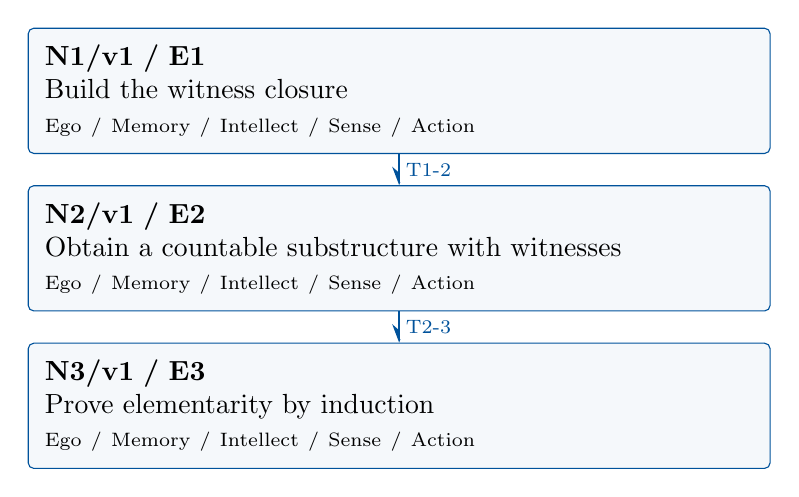
\begin{tikzpicture}[>=Stealth,x=1cm,y=1cm]

\node[mmnode,text width=9cm,minimum height=1.25cm] (N1) at (0,0.0) {\textbf{N1/v1 / E1}\\Build the witness closure\\{\scriptsize Ego / Memory / Intellect / Sense / Action}};

\node[mmnode,text width=9cm,minimum height=1.25cm] (N2) at (0,-2.0) {\textbf{N2/v1 / E2}\\Obtain a countable substructure with witnesses\\{\scriptsize Ego / Memory / Intellect / Sense / Action}};

\node[mmnode,text width=9cm,minimum height=1.25cm] (N3) at (0,-4.0) {\textbf{N3/v1 / E3}\\Prove elementarity by induction\\{\scriptsize Ego / Memory / Intellect / Sense / Action}};

\draw[mmproof] (N1.south) -- node[mmnote,right] {T1-2} (N2.north);

\draw[mmproof] (N2.south) -- node[mmnote,right] {T2-3} (N3.north);

\end{tikzpicture}\end{center}

Each box is one mathematical agent containing all five faculties. Blue
arrows carry the versioned exports listed below. The layout gives a
reading order; only drawn arrows assert dependencies. Diagnostic repair
is separate from the proof DAG.

\subsection{Versioned evidence-transfer ledger}

\begingroup\small\linespread{1.05}\selectfont

\Needspace{5\baselineskip}\field{T1-2: N1/E1/v1 to N2}{There are increasing countable sets \(B_n\) such that \(B_{n+1}\)
contains all function values on \(B_n\) and witnesses for all true
existential formulas with parameters in \(B_n\).}

\field{Receiving activity}{N2.1}

\field{Compatibility}{E1/v1 and \(B=\bigcup_{n\ge0}B_n\). Check: Closure under functions alone
is insufficient for elementarity; retain the existential witness closure
as a distinct export.}

\Needspace{5\baselineskip}\field{T2-3: N2/E2/v1 to N3}{The restricted structure \(N\) on \(B\) is countable, contains \(A\),
and every existential formula true in \(M\) with parameters in \(N\) has
a witness in \(N\).}

\field{Receiving activity}{N3.1}

\field{Compatibility}{E2/v1 and recursive first-order semantics. Check: An existential witness
true in \(M\) must be transferred using the induction hypothesis for its
matrix, not simply declared true in \(N\).}

\endgroup

\clearpage\section{Agent roles and five-faculty activities}\begingroup\small\linespread{1.05}\selectfont\setlist{itemsep=1pt,topsep=2pt}

\begingroup\footnotesize\linespread{1.05}\selectfont\let\small\footnotesize

\subsection{N1/v1: Build the witness closure}

\field{Object and role}{At each stage add function values and one witness for each true
existential formula over the current parameter set. \textbf{Local
obligation:} There are increasing countable sets \(B_n\) such that
\(B_{n+1}\) contains all function values on \(B_n\) and witnesses for
all true existential formulas with parameters in \(B_n\).}

\field{Inputs}{A countable seed \(B_0\supset A\) containing one element of \(M\), and
all formulas and language symbols.}

\mmfaculty{E}{Ego}{Publish E1/v1 only after establishing this obligation: There are
increasing countable sets \(B_n\) such that \(B_{n+1}\) contains all
function values on \(B_n\) and witnesses for all true existential
formulas with parameters in \(B_n\).}

\mmfaculty{M}{Memory}{A countable seed \(B_0\supset A\) containing one element of \(M\), and
all formulas and language symbols. Retain the stated assumptions and
import versions.}

\mmfaculty{I}{Intellect}{At each stage add function values and one witness for each true
existential formula over the current parameter set.}

\mmfaculty{S}{Sense}{Each stage makes only countably many requests; parameters added later
require new stages.}

\mmfaculty{A}{Action}{Carry out activities N1.1--N1.2 below, retaining each calculation and
construction as evidence.}

\smallskip\noindent\textbf{Numbered mathematical activities}

\begin{enumerate}[label=N1.\arabic*,leftmargin=3.4em]

\item Choose one element of \(M\) and adjoin it to \(A\) to make \(B_0\)
nonempty. Given \(B_n\), include in \(B_{n+1}\) the interpretations of
all constants and of all finite-arity function symbols applied to tuples
from \(B_n\). There are countably many such requests.

\item Also list every existential formula \(\exists x\,\psi(x,\bar b)\) with a
finite tuple \(\bar b\) from \(B_n\) that is true in \(M\). There are
countably many formulas and parameter tuples. Choose one witness in
\(M\) for each true request and add it. With \(B_n\) itself included,
the result remains countable and the construction can be repeated.

\end{enumerate}

\field{Export E1/v1}{There are increasing countable sets \(B_n\) such that \(B_{n+1}\)
contains all function values on \(B_n\) and witnesses for all true
existential formulas with parameters in \(B_n\).}

\field{Acceptance gate}{Each stage makes only countably many requests; parameters added later
require new stages.}

\field{Targeted repair}{If closure is performed just once, repeat it through all natural-number
stages so formulas involving newly added witnesses are covered. Withhold
this export and recheck its descendants after a versioned correction.}

\endgroup

\clearpage

\subsection{N2/v1: Obtain a countable substructure with witnesses}

\field{Object and role}{Use finiteness of parameter tuples to locate all their entries in one
stage. \textbf{Local obligation:} The restricted structure \(N\) on
\(B\) is countable, contains \(A\), and every existential formula true
in \(M\) with parameters in \(N\) has a witness in \(N\).}

\field{Inputs}{E1/v1 and \(B=\bigcup_{n\ge0}B_n\). Incoming proof exports: E1/v1 at
N2.1.}

\mmfaculty{E}{Ego}{Publish E2/v1 only after establishing this obligation: The restricted
structure \(N\) on \(B\) is countable, contains \(A\), and every
existential formula true in \(M\) with parameters in \(N\) has a witness
in \(N\).}

\mmfaculty{M}{Memory}{E1/v1 and \(B=\bigcup_{n\ge0}B_n\). Incoming proof exports: E1/v1 at
N2.1. Retain the stated assumptions and import versions.}

\mmfaculty{I}{Intellect}{Use finiteness of parameter tuples to locate all their entries in one
stage.}

\mmfaculty{S}{Sense}{Closure under functions alone is insufficient for elementarity; retain
the existential witness closure as a distinct export.}

\mmfaculty{A}{Action}{Carry out activities N2.1--N2.2 below, retaining each calculation and
construction as evidence.}

\smallskip\noindent\textbf{Numbered mathematical activities}

\begin{enumerate}[label=N2.\arabic*,leftmargin=3.4em]

\item The union \(B\) is nonempty and at most countable. Any finite tuple from
\(B\) lies entirely in some \(B_n\), so each language function evaluated
there lies in \(B_{n+1}\subset B\). Constants also lie in \(B\). Thus
restriction defines an \(L\)-substructure \(N\) containing \(A\).

\item If \(M\models\exists x\,\psi(x,\bar b)\) with \(\bar b\) in \(B\),
choose a stage containing the whole finite tuple. N1 added a witness at
the next stage. Hence such a witness is in \(B\), with the matrix
formula true in \(M\). This is the precise witness property needed next.

\end{enumerate}

\field{Export E2/v1}{The restricted structure \(N\) on \(B\) is countable, contains \(A\),
and every existential formula true in \(M\) with parameters in \(N\) has
a witness in \(N\).}

\field{Acceptance gate}{Closure under functions alone is insufficient for elementarity; retain
the existential witness closure as a distinct export.}

\field{Targeted repair}{If the proof assumes the union is closed under an operation with
infinitely many arguments, restore the finite-arity language contract;
the common-stage argument depends on it. Withhold this export and
recheck its descendants after a versioned correction.}

\clearpage

\begingroup\footnotesize\linespread{1.05}\selectfont\let\small\footnotesize

\subsection{N3/v1: Prove elementarity by induction}

\field{Object and role}{Induct through atomic formulas, Boolean operations, and existential
quantification in both directions. \textbf{Local obligation:}
\(N\preccurlyeq M\); if \(M\) is infinite, \(N\) is countably infinite.}

\field{Inputs}{E2/v1 and recursive first-order semantics. Incoming proof exports: E2/v1
at N3.1.}

\mmfaculty{E}{Ego}{Publish E3/v1 only after establishing this obligation:
\(N\preccurlyeq M\); if \(M\) is infinite, \(N\) is countably infinite.}

\mmfaculty{M}{Memory}{E2/v1 and recursive first-order semantics. Incoming proof exports: E2/v1
at N3.1. Retain the stated assumptions and import versions.}

\mmfaculty{I}{Intellect}{Induct through atomic formulas, Boolean operations, and existential
quantification in both directions.}

\mmfaculty{S}{Sense}{An existential witness true in \(M\) must be transferred using the
induction hypothesis for its matrix, not simply declared true in \(N\).}

\mmfaculty{A}{Action}{Carry out activities N3.1--N3.3 below, retaining each calculation and
construction as evidence.}

\smallskip\noindent\textbf{Numbered mathematical activities}

\begin{enumerate}[label=N3.\arabic*,leftmargin=3.4em]

\item Terms evaluate identically in \(N\) and \(M\) on tuples from \(N\), by
induction and function restriction. Atomic equalities and relations
therefore agree. If formulas agree, their negations and conjunctions
agree by the same truth tables.

\item For an existential formula, a witness in \(N\) makes its matrix true in
\(M\) by the induction hypothesis, proving the forward implication.
Conversely, if the existential formula is true in \(M\), E2 supplies a
witness in \(N\) whose matrix is true in \(M\); the induction hypothesis
makes that matrix true in \(N\). Thus the existential formula is true in
\(N\). This completes the induction for all formulas and proves
elementarity.

\item If \(M\) is infinite, for every positive integer \(r\) it satisfies the
sentence asserting \(r\) pairwise distinct elements. Elementarity
transfers each such sentence to \(N\), so \(N\) is infinite. Since it is
at most countable, it is countably infinite.

\end{enumerate}

\field{Export E3/v1}{\(N\preccurlyeq M\); if \(M\) is infinite, \(N\) is countably infinite.}

\field{Acceptance gate}{An existential witness true in \(M\) must be transferred using the
induction hypothesis for its matrix, not simply declared true in \(N\).}

\field{Targeted repair}{If elementarity is inferred from function closure, add the witness
property and the two directions of the existential induction;
substructure alone does not imply elementary substructure. Withhold this
export and recheck its descendants after a versioned correction.}

\endgroup

\endgroup\clearpage\section{Continuous mathematical proof}\label{sec:proof}

\subsection{N1 --- Build the witness
closure}\label{n1-build-the-witness-closure}

\begin{enumerate}
\def\labelenumi{\arabic{enumi}.}
\item
  \textbf{N1.1.} Choose one element of \(M\) and adjoin it to \(A\) to
  make \(B_0\) nonempty. Given \(B_n\), include in \(B_{n+1}\) the
  interpretations of all constants and of all finite-arity function
  symbols applied to tuples from \(B_n\). There are countably many such
  requests.
\item
  \textbf{N1.2.} Also list every existential formula
  \(\exists x\,\psi(x,\bar b)\) with a finite tuple \(\bar b\) from
  \(B_n\) that is true in \(M\). There are countably many formulas and
  parameter tuples. Choose one witness in \(M\) for each true request
  and add it. With \(B_n\) itself included, the result remains countable
  and the construction can be repeated.
\end{enumerate}

\subsection{N2 --- Obtain a countable substructure with
witnesses}\label{n2-obtain-a-countable-substructure-with-witnesses}

\begin{enumerate}
\def\labelenumi{\arabic{enumi}.}
\item
  \textbf{N2.1.} The union \(B\) is nonempty and at most countable. Any
  finite tuple from \(B\) lies entirely in some \(B_n\), so each
  language function evaluated there lies in \(B_{n+1}\subset B\).
  Constants also lie in \(B\). Thus restriction defines an
  \(L\)-substructure \(N\) containing \(A\).
\item
  \textbf{N2.2.} If \(M\models\exists x\,\psi(x,\bar b)\) with
  \(\bar b\) in \(B\), choose a stage containing the whole finite tuple.
  N1 added a witness at the next stage. Hence such a witness is in
  \(B\), with the matrix formula true in \(M\). This is the precise
  witness property needed next.
\end{enumerate}

\subsection{N3 --- Prove elementarity by
induction}\label{n3-prove-elementarity-by-induction}

\begin{enumerate}
\def\labelenumi{\arabic{enumi}.}
\item
  \textbf{N3.1.} Terms evaluate identically in \(N\) and \(M\) on tuples
  from \(N\), by induction and function restriction. Atomic equalities
  and relations therefore agree. If formulas agree, their negations and
  conjunctions agree by the same truth tables.
\item
  \textbf{N3.2.} For an existential formula, a witness in \(N\) makes
  its matrix true in \(M\) by the induction hypothesis, proving the
  forward implication. Conversely, if the existential formula is true in
  \(M\), E2 supplies a witness in \(N\) whose matrix is true in \(M\);
  the induction hypothesis makes that matrix true in \(N\). Thus the
  existential formula is true in \(N\). This completes the induction for
  all formulas and proves elementarity.
\item
  \textbf{N3.3.} If \(M\) is infinite, for every positive integer \(r\)
  it satisfies the sentence asserting \(r\) pairwise distinct elements.
  Elementarity transfers each such sentence to \(N\), so \(N\) is
  infinite. Since it is at most countable, it is countably infinite.
\end{enumerate}

\hfill$\square$

\section{Worked orchestration}

Apply the construction to \((\mathbb R,+,\cdot,<,0,1)\) with seed
\(A=\mathbb Q\). The true formula \(\exists x\,(x>0\wedge x^2=2)\)
demands a witness, so the closure adds \(\sqrt2\). Repeated stages
supply witnesses for all formulas over the growing set. The resulting
countable elementary substructure is more than the initial rational
field; the construction does not assert that it equals a particular
named subfield.

\subsection{Boundary and hypothesis audit}

The subfield \(\mathbb Q\subset\mathbb R\) is a substructure of ordered
fields but not an elementary substructure, because
\(\exists x\,(x^2=2)\) is false in \(\mathbb Q\) and true in
\(\mathbb R\). Countability of the language also matters: if a distinct
constant names every element of an uncountable structure, every
substructure must contain all those named elements.

\section{Illustrative failure and repair}

The following is an authored diagnostic scenario. Changed assumptions
define a new contract; they do not retroactively prove the original
statement.

\subsection{Rejected argument, diagnosis, and correction}
\textbf{Rejected N2 conclusion:} closing the seed under field operations
is enough. Starting with \(\mathbb Q\) leaves \(\mathbb Q\), which fails
the square-root existential sentence. \textbf{Diagnosis:} Memory
recorded function closure but omitted existential witnesses.
\textbf{Repair:} add one witness for every true existential request at
every stage, then prove formula agreement by N3. The original theorem
and seed are preserved; recheck countability and the elementarity
induction.

\subsection{Publication and reuse}
The corrected export retains its explicit assumptions. A hypothetical
revision receives a new version, and each consuming activity is
rechecked; this scenario is not a recorded runtime event. \textbf{Next
direction:} Explore the distinction between internal and external
countability in models of set theory, without interpreting the theorem
as a contradiction about cardinality.

\par\medskip\begingroup\small\linespread{1.0}\selectfont\noindent\textbf{Provenance.} This authored proof is complete relative to its declared imports. Reuse
each export with its assumptions, proof, and version. The original
Markdown remains available for comparison.
\par\endgroup

\par\smallskip\begingroup\small\linespread{1.0}\selectfont\noindent\textbf{Further reading.} \href{https://math.berkeley.edu/~marks/notes/set_theory_notes_4.pdf}{Andrew
Marks, Set Theory notes} for sets and ultraproducts;
\href{https://math.berkeley.edu/~antonio/math125A/mathlogicP1.pdf}{Berkeley,
Mathematical Logic for Mathematicians, Part I} for first-order
semantics;
\href{https://math.berkeley.edu/~marks/notes/computability_notes_v1.pdf}{Andrew
Marks, Computability Theory notes} for effective procedures and
undecidability. The proofs below specify their own set-theoretic and
semantic assumptions.\par\endgroup

\end{document}
